\documentclass{standalone}
\usepackage{tikz}
\usetikzlibrary{patterns, positioning}
\usepackage[sfdefault]{ClearSans} %% option 'sfdefault' activates Clear Sans as the default text font
\usepackage[T1]{fontenc}

\begin{document}
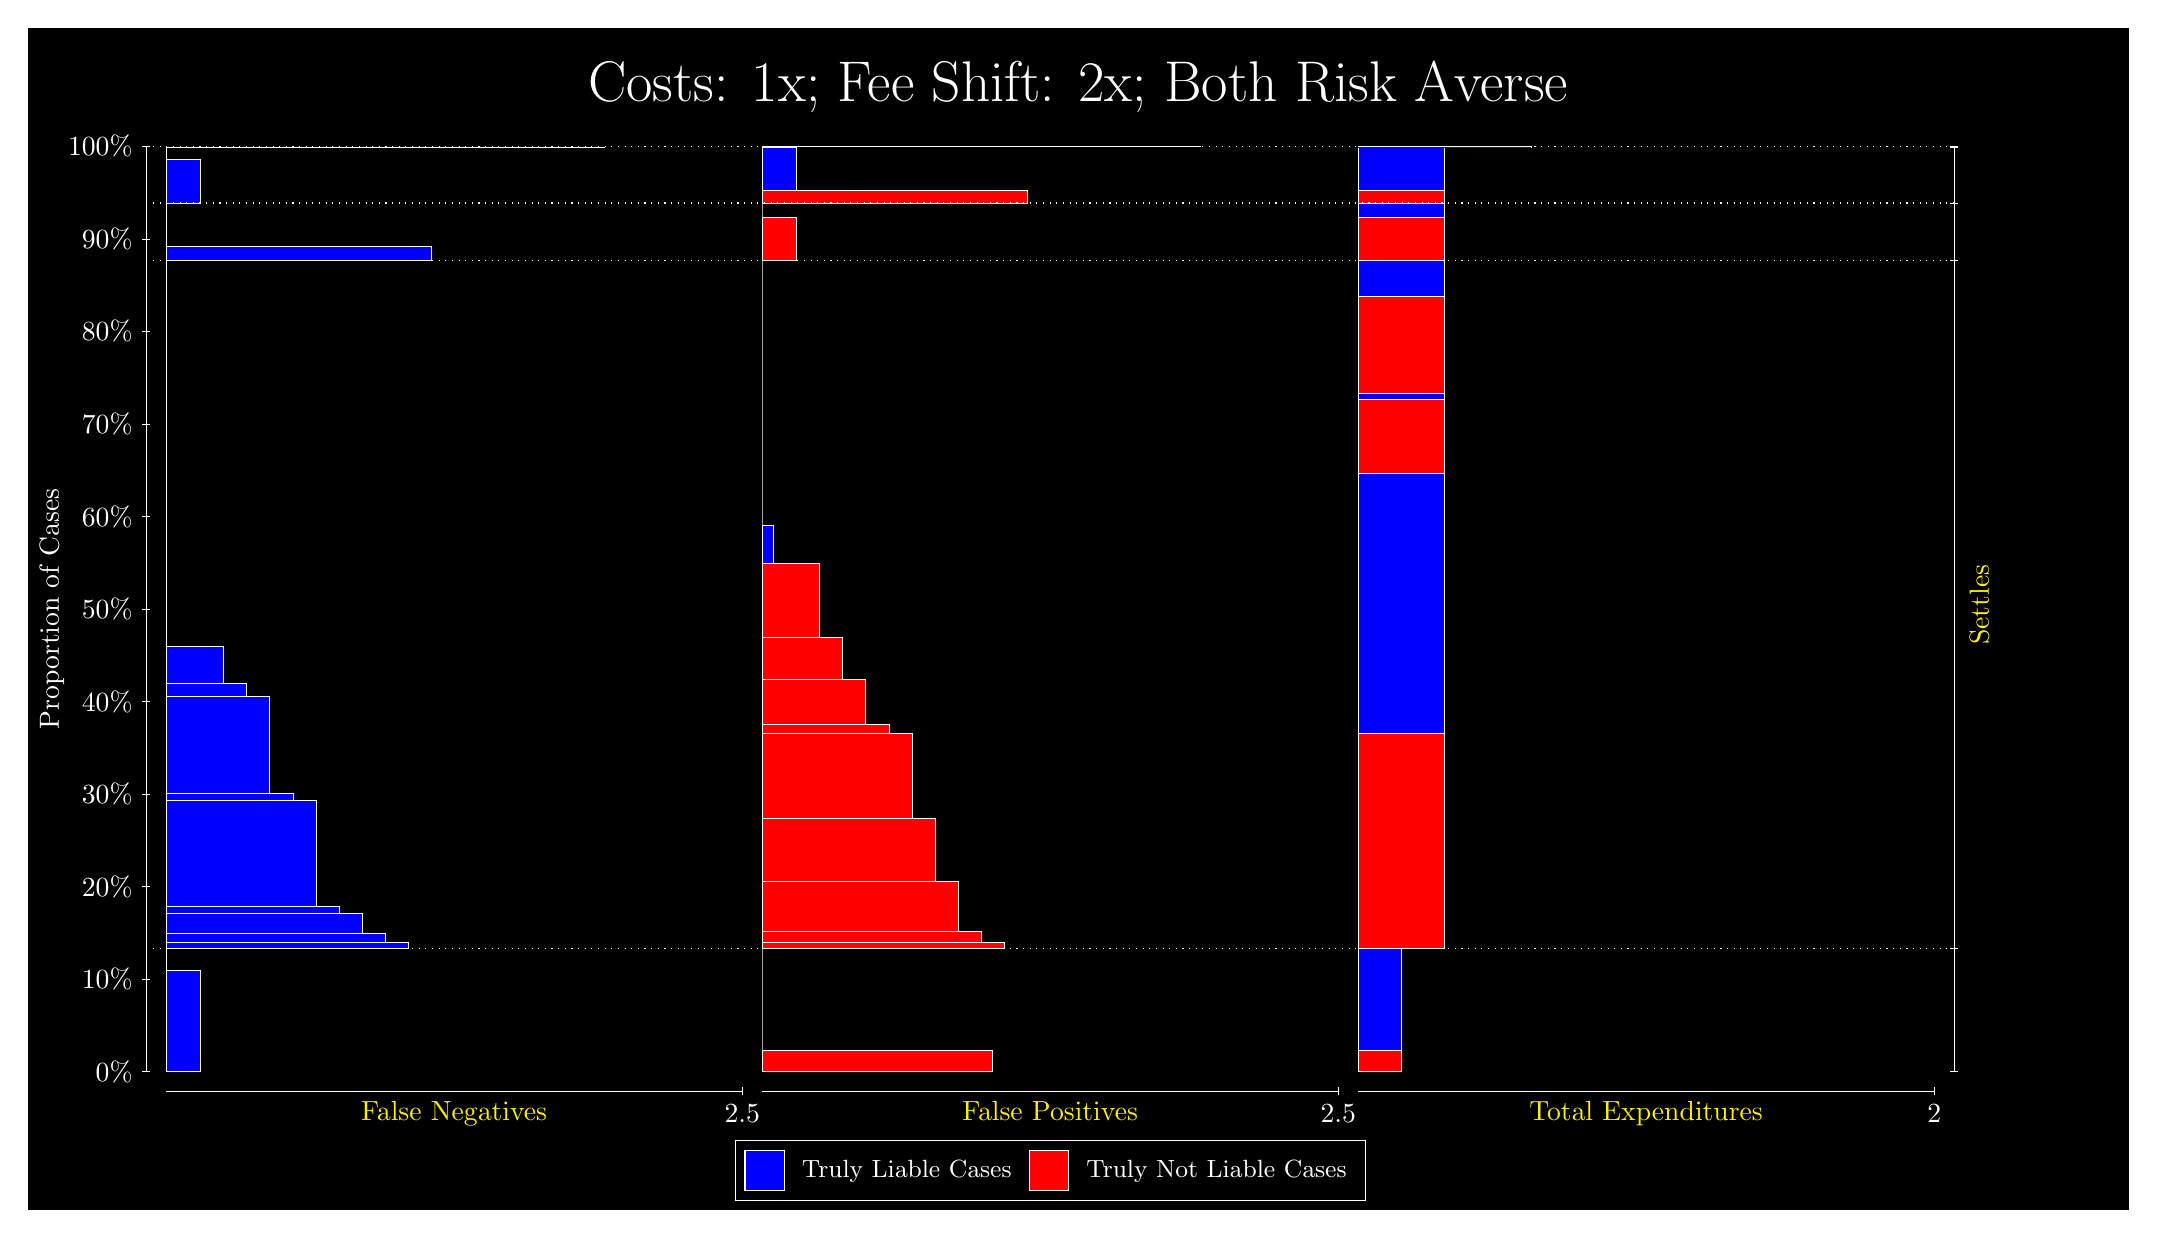
\begin{tikzpicture}
\draw[fill=black] (0,0) rectangle (26.667,15);
\draw[text=white] (0,13.5) rectangle (26.667,15) node[midway] {\huge Costs: 1x; Fee Shift: 2x; Both Risk Averse};
\draw[white, very thin] (1.5,1.75) -- (1.5,13.5);
\node[rotate=90, text=white, anchor=center] at (0.3, 7.625) {Proportion of Cases};
\draw[white, very thin] (1.45,1.75) -- (1.55,1.75);
\node[text=white, anchor=east] at (1.45, 1.75) {0\%};
\draw[white, very thin] (1.45,2.925) -- (1.55,2.925);
\node[text=white, anchor=east] at (1.45, 2.925) {10\%};
\draw[white, very thin] (1.45,4.1) -- (1.55,4.1);
\node[text=white, anchor=east] at (1.45, 4.1) {20\%};
\draw[white, very thin] (1.45,5.275) -- (1.55,5.275);
\node[text=white, anchor=east] at (1.45, 5.275) {30\%};
\draw[white, very thin] (1.45,6.45) -- (1.55,6.45);
\node[text=white, anchor=east] at (1.45, 6.45) {40\%};
\draw[white, very thin] (1.45,7.625) -- (1.55,7.625);
\node[text=white, anchor=east] at (1.45, 7.625) {50\%};
\draw[white, very thin] (1.45,8.8) -- (1.55,8.8);
\node[text=white, anchor=east] at (1.45, 8.8) {60\%};
\draw[white, very thin] (1.45,9.975) -- (1.55,9.975);
\node[text=white, anchor=east] at (1.45, 9.975) {70\%};
\draw[white, very thin] (1.45,11.15) -- (1.55,11.15);
\node[text=white, anchor=east] at (1.45, 11.15) {80\%};
\draw[white, very thin] (1.45,12.325) -- (1.55,12.325);
\node[text=white, anchor=east] at (1.45, 12.325) {90\%};
\draw[white, very thin] (1.45,13.5) -- (1.55,13.5);
\node[text=white, anchor=east] at (1.45, 13.5) {100\%};

\draw[white, very thin] (24.457,1.75) -- (24.457,13.5);
\draw[white, very thin] (24.407,1.75) -- (24.507,1.75);
\node[anchor=west] at (24.407, 1.75) {};
\draw[white, very thin] (24.407,3.3106) -- (24.507,3.3106);
\node[anchor=west] at (24.407, 3.3106) {};
\draw[white, very thin] (24.407,12.048) -- (24.507,12.048);
\node[anchor=west] at (24.407, 12.048) {};
\draw[white, very thin] (24.407,12.78) -- (24.507,12.78);
\node[anchor=west] at (24.407, 12.78) {};
\draw[white, very thin] (24.407,13.493) -- (24.507,13.493);
\node[anchor=west] at (24.407, 13.493) {};
\draw[white, very thin] (24.407,13.496) -- (24.507,13.496);
\node[anchor=west] at (24.407, 13.496) {};
\draw[white, very thin] (24.407,13.5) -- (24.507,13.5);
\node[anchor=west] at (24.407, 13.5) {};

\draw[white, very thin, fill=blue] (1.75,1.75) rectangle (2.1891,3.042);
\draw[white, very thin, fill=red] (1.75,3.042) rectangle (1.75,3.3106);
\draw[white, very thin, fill=blue] (1.75,3.3106) rectangle (4.8239,3.3924);
\draw[white, very thin, fill=blue] (1.75,3.3924) rectangle (4.5312,3.509);
\draw[white, very thin, fill=blue] (1.75,3.509) rectangle (4.2384,3.7583);
\draw[white, very thin, fill=blue] (1.75,3.7583) rectangle (3.9457,3.8491);
\draw[white, very thin, fill=blue] (1.75,3.8491) rectangle (3.6529,5.1909);
\draw[white, very thin, fill=blue] (1.75,5.1909) rectangle (3.3602,5.2872);
\draw[white, very thin, fill=blue] (1.75,5.2872) rectangle (3.0674,6.5167);
\draw[white, very thin, fill=blue] (1.75,6.5167) rectangle (2.7746,6.677);
\draw[white, very thin, fill=blue] (1.75,6.677) rectangle (2.4819,7.1534);
\draw[white, very thin, fill=red] (1.75,7.1534) rectangle (1.75,12.048);
\draw[white, very thin, fill=blue] (1.75,12.048) rectangle (5.1167,12.228);
\draw[white, very thin, fill=red] (1.75,12.228) rectangle (1.75,12.78);
\draw[white, very thin, fill=blue] (1.75,12.78) rectangle (2.1891,13.337);
\draw[white, very thin, fill=red] (1.75,13.337) rectangle (1.75,13.493);
\draw[white, very thin, fill=blue] (1.75,13.493) rectangle (7.3123,13.494);
\draw[white, very thin, fill=red] (1.75,13.494) rectangle (1.75,13.496);
\draw[white, very thin, fill=red] (1.75,13.496) rectangle (1.75,13.498);
\draw[white, very thin, fill=blue] (1.75,13.498) rectangle (1.75,13.5);
\draw[white, very thin, fill=red] (9.3189,1.75) rectangle (12.246,2.0186);
\draw[white, very thin, fill=blue] (9.3189,2.0186) rectangle (9.3189,3.3106);
\draw[white, very thin, fill=red] (9.3189,3.3106) rectangle (12.393,3.3874);
\draw[white, very thin, fill=red] (9.3189,3.3874) rectangle (12.1,3.5375);
\draw[white, very thin, fill=red] (9.3189,3.5375) rectangle (11.807,4.1645);
\draw[white, very thin, fill=red] (9.3189,4.1645) rectangle (11.515,4.9721);
\draw[white, very thin, fill=red] (9.3189,4.9721) rectangle (11.222,6.0418);
\draw[white, very thin, fill=red] (9.3189,6.0418) rectangle (10.929,6.1646);
\draw[white, very thin, fill=red] (9.3189,6.1646) rectangle (10.636,6.7326);
\draw[white, very thin, fill=red] (9.3189,6.7326) rectangle (10.344,7.2671);
\draw[white, very thin, fill=red] (9.3189,7.2671) rectangle (10.051,8.2054);
\draw[white, very thin, fill=blue] (9.3189,8.2054) rectangle (9.4652,8.6817);
\draw[white, very thin, fill=blue] (9.3189,8.6817) rectangle (9.3189,12.048);
\draw[white, very thin, fill=red] (9.3189,12.048) rectangle (9.758,12.601);
\draw[white, very thin, fill=blue] (9.3189,12.601) rectangle (9.3189,12.78);
\draw[white, very thin, fill=red] (9.3189,12.78) rectangle (12.686,12.936);
\draw[white, very thin, fill=blue] (9.3189,12.936) rectangle (9.758,13.493);
\draw[white, very thin, fill=red] (9.3189,13.493) rectangle (9.3189,13.495);
\draw[white, very thin, fill=blue] (9.3189,13.495) rectangle (9.3189,13.496);
\draw[white, very thin, fill=red] (9.3189,13.496) rectangle (14.881,13.498);
\draw[white, very thin, fill=blue] (9.3189,13.498) rectangle (11.954,13.5);
\draw[white, very thin, fill=red] (16.888,1.75) rectangle (17.437,2.0186);
\draw[white, very thin, fill=blue] (16.888,2.0186) rectangle (17.437,3.3106);
\draw[white, very thin, fill=red] (16.888,3.3106) rectangle (17.986,6.0418);
\draw[white, very thin, fill=blue] (16.888,6.0418) rectangle (17.986,9.3461);
\draw[white, very thin, fill=red] (16.888,9.3461) rectangle (17.986,10.284);
\draw[white, very thin, fill=blue] (16.888,10.284) rectangle (17.986,10.366);
\draw[white, very thin, fill=red] (16.888,10.366) rectangle (17.986,11.591);
\draw[white, very thin, fill=blue] (16.888,11.591) rectangle (17.986,12.048);
\draw[white, very thin, fill=red] (16.888,12.048) rectangle (17.986,12.601);
\draw[white, very thin, fill=blue] (16.888,12.601) rectangle (17.986,12.78);
\draw[white, very thin, fill=red] (16.888,12.78) rectangle (17.986,12.936);
\draw[white, very thin, fill=blue] (16.888,12.936) rectangle (17.986,13.493);
\draw[white, very thin, fill=red] (16.888,13.493) rectangle (19.083,13.495);
\draw[white, very thin, fill=blue] (16.888,13.495) rectangle (19.083,13.496);
\draw[white, very thin, fill=red] (16.888,13.496) rectangle (19.083,13.498);
\draw[white, very thin, fill=blue] (16.888,13.498) rectangle (19.083,13.5);
\draw[white, dotted] (1.5,3.3106) -- (24.457,3.3106);
\draw[white, dotted] (1.5,12.048) -- (24.457,12.048);
\draw[white, dotted] (1.5,12.78) -- (24.457,12.78);
\draw[white, dotted] (1.5,13.493) -- (24.457,13.493);
\draw[white, dotted] (1.5,13.496) -- (24.457,13.496);
\draw[white, very thin] (1.75,1.5) -- (9.0689,1.5);
\node[text=yellow, anchor=north] at (5.4094, 1.5) {False Negatives};
\draw[white, very thin] (9.0689,1.45) -- (9.0689,1.55);
\node[text=white, anchor=north] at (9.0689, 1.45) {2.5};

\draw[white, very thin] (9.3189,1.5) -- (16.638,1.5);
\node[text=yellow, anchor=north] at (12.978, 1.5) {False Positives};
\draw[white, very thin] (16.638,1.45) -- (16.638,1.55);
\node[text=white, anchor=north] at (16.638, 1.45) {2.5};

\draw[white, very thin] (16.888,1.5) -- (24.207,1.5);
\node[text=yellow, anchor=north] at (20.547, 1.5) {Total Expenditures};
\draw[white, very thin] (24.207,1.45) -- (24.207,1.55);
\node[text=white, anchor=north] at (24.207, 1.45) {2};


\node[text=yellow, centered, rotate=90] at (24.777, 7.6794) {Settles};





\draw (12.978300999999998,1.5) node[draw=none] (baseCoordinate) {};
\begin{scope}[align=center]
        \matrix[scale=0.5, draw=white, below=0.5cm of baseCoordinate, nodes={draw}, column sep=0.1cm]{
            \node[rectangle, draw, minimum width=0.5cm, minimum height=0.5cm, fill=blue] {}; &
            \node[draw=none, font=\small, text=white] (B) {Truly Liable Cases}; &
            \node[rectangle, draw, minimum width=0.5cm, minimum height=0.5cm, fill=red] {}; &
            \node[draw=none, font=\small, text=white] (B) {Truly Not Liable Cases}; \\
            };
\end{scope}

\end{tikzpicture}
\end{document}